\documentclass[11pt,a4paper]{article}
\usepackage[utf8]{inputenc}
\usepackage[T1]{fontenc}
\usepackage{lmodern}
\usepackage{microtype}
\usepackage[margin=1in]{geometry}
\usepackage{graphicx}
\usepackage{booktabs}
\usepackage{hyperref}
\usepackage{xcolor}
\usepackage{listings}
\hypersetup{colorlinks=true,linkcolor=blue,urlcolor=blue,citecolor=blue}

\lstset{
  basicstyle=\ttfamily\small,
  breaklines=true,
  frame=single,
  framerule=0pt,
  backgroundcolor=\color{gray!10},
  showstringspaces=false,
}

\title{ACP: Intent-Resolved Execution Manifests for Production Agent Systems}
\author{Shreyansh Sancheti\\
        \texttt{shreyansh@clawdlinux.org}\\
        Clawdlinux / NineVigil}
\date{Draft updated 2026-05-13}

\begin{document}
\maketitle

\begin{abstract}
Production agent systems built on the Model Context Protocol (MCP) spend the
majority of their context window on tool discovery and verbose JSON-Schema
descriptors before performing any user task. We measure this overhead at
64.7\%-97.4\% across five representative workflows using committed,
reproducible payloads. We introduce the
\textbf{Agent Context Protocol (ACP)}, a layer that sits \emph{on top of} MCP
and other tool sources and returns a single intent-scoped Execution Manifest
in one round trip with auth pre-injected, dependency order pre-computed, and
security boundaries declared. ACP cuts tool-context tokens by 64.7\%-97.4\%
(mean 76.6\%) and reduces round trips before the first useful action from
3-21 to 1, while preserving the underlying MCP ecosystem unchanged. Unlike
schema-only compression libraries or agent-side active discovery, ACP combines
server-side intent resolution, schema stripping, credential injection, and
dependency pre-computation into one execution manifest. We provide an
open-source reference implementation in Go with a Python adapter suite for
OpenAI-compatible function calling, LangGraph, and CrewAI; the protocol
specification is published under CC BY 4.0 and the SDKs under Apache 2.0.
\end{abstract}

\section{Introduction}

Autonomous AI agents increasingly orchestrate work across many tools exposed
by Model Context Protocol (MCP) servers~\cite{mcp}. The protocol's design
centers on tool discoverability: every connected MCP server publishes a
\texttt{tools/list} response that the agent loads in full at the start of
each session. This is appropriate for human-in-the-loop browsing of tool
catalogs; it is poorly suited to the production case where an agent is
given a specific intent and a context-window budget.

Prior measurement work~\cite{eckstein2025,apideck2025,scalekit2026} documents
that real MCP deployments routinely consume the majority of the agent's
context window with tool descriptors before the user's task begins. We
replicate and extend those measurements in a controlled benchmark
(Section~\ref{sec:eval}).

We argue that the right intervention is \emph{not} to replace MCP, but to
add a thin layer above it that resolves the agent's intent, compacts the
verbose tool descriptors, injects credentials at a proxy boundary, and
returns the resulting Execution Manifest in a single HTTP round trip. The
MCP ecosystem (servers, registries, tooling) remains unchanged.

\section{Background and Related Work}

\textbf{MCP}~\cite{mcp} is a JSON-RPC protocol that lets agents discover and
invoke tools published by independent servers. Its \texttt{tools/list}
response carries the full JSON-Schema for each tool's input parameters,
including descriptions, examples, and constraint metadata.

\textbf{Tool-schema compression.} TSCG~\cite{sakizli2026tscg} is the closest
schema-level comparison. It deterministically compiles JSON tool schemas into
token-efficient structured text at the API boundary and reports 52\%-57\%
token savings across model and schema settings. ACP uses schema stripping as
one component, but differs in where the decision is made and what is returned:
ACP is a server-side protocol that first resolves an intent to a small tool
subset, then returns an execution manifest with auth and ordering metadata.
TSCG compresses the schemas supplied to it; ACP also decides which schemas
should not be supplied at all.

\textbf{Active discovery.} MCP-Zero~\cite{fei2025mcpzero} reduces context
overhead by letting the model request tools on demand through hierarchical
semantic routing and iterative capability extension. ACP takes the opposite
deployment stance: discovery autonomy is moved out of the model loop and into
a server layer. The agent sends one intent and receives one manifest, instead
of spending model turns assembling a toolchain.

\textbf{MCP description quality.} Hasan et al.~\cite{hasan2026smelly} find
that 97.1\% of 856 tool descriptions across 103 MCP servers contain at least
one quality defect, and that augmenting descriptions can improve success while
also increasing execution cost. This work supports the observation that tool
descriptors are load-bearing context, but it optimizes description quality
within MCP rather than reducing the structural cost of loading irrelevant
tools.

\textbf{Code-oriented alternatives.} Cloudflare Code Mode~\cite{cfcodemode}
sidesteps descriptor cost by having agents emit code against typed SDKs. The
reduction is substantial but requires the agent to be a code-generating model
and the deployment to be on Cloudflare.

\textbf{A2A Agent Cards}~\cite{a2a} expose
\texttt{/.well-known/agent-card.json} for inter-agent discovery. They solve
``what agents exist'' rather than ``how should this agent execute now.''

\textbf{Agent manifests and interoperability.} AgentSpec~\cite{agentspec} is
a declarative manifest for an \emph{agent's} configuration, dependency checks,
policy, and observability. ACP is orthogonal: AgentSpec describes the agent
itself; ACP describes one execution context for one task. An agent
interoperability survey~\cite{ehtesham2025interop} also uses the acronym ACP
for IBM's Agent Communication Protocol, a RESTful agent-to-agent messaging
protocol. In this paper, ACP means \textbf{Agent Context Protocol}, a
tool-context optimization protocol rather than an agent-to-agent messaging
protocol.

\textbf{Oracle Open Agent Spec}~\cite{oracleopenagent} is a design-time
workflow language for multi-agent systems. ACP operates at runtime, scoped
to a single intent.

\textbf{Open tool-use benchmarks.} BFCL~\cite{patil2025bfcl} provides an
open, citable function-calling benchmark with executable correctness checks
and model leaderboards. tau-bench~\cite{yao2024taubench} evaluates multi-turn
tool-agent-user interaction. ACP's current evaluation is a protocol-overhead
benchmark; the next benchmark track maps BFCL-style function sets into MCP and
ACP payloads to measure context overhead, tool-call correctness, cost, and
latency across model tiers.

\section{Protocol}

\subsection{Wire format}

An ACP request is one HTTP POST:

\begin{lstlisting}
POST /v1/context
Content-Type: application/json
Authorization: Bearer <agent-identity-token>

{
  "intent": "query customer data, send a slack notification",
  "agent_id": "analytics-agent-01",
  "capabilities": ["sql", "messaging"]
}
\end{lstlisting}

The response is one Execution Manifest with a small list of typed
\texttt{actions}, each carrying a compacted \texttt{schema}, an opaque
\texttt{auth: pre-injected} marker, and an optional \texttt{depends\_on}
array.

\subsection{Schema mini-language}

ACP compacts JSON-Schema input parameters into a typed mini-language:
\texttt{string}, \texttt{int?}, \texttt{string[]},
\texttt{enum:open|closed}, \texttt{ref:<id>}. This preserves executable
meaning while removing prose descriptions, examples, and constraint
metadata. The compaction is the source of the token reduction reported in
Section~\ref{sec:eval}.

\subsection{Auth injection}

The manifest's \texttt{auth} field is always \texttt{pre-injected}. The
accompanying ACP auth proxy mounts at
\texttt{/v1/exec/\{manifest\_id\}/\{action\_id\}} and forwards each action
to the upstream tool with credentials added at the proxy boundary. The
agent never receives or stores credentials.

\subsection{Relationship to MCP}

ACP does not modify or replace MCP. The reference implementation includes
an MCP source adapter that consumes an upstream MCP server's
\texttt{tools/list} payload, infers ACP capability tags from each tool's
name, compacts the JSON-Schema input parameters to the mini-language, and
registers each tool in the ACP registry. Existing MCP servers are
unmodified.

\section{Evaluation}\label{sec:eval}

\subsection{Setup}

We compare two paths for the same five workflows. The MCP path is the
verbose \texttt{initialize} + \texttt{tools/list} payload an agent must
keep in context to invoke the tools, built per the MCP 2024-11
specification with the same descriptors a real server would return. The
ACP path is the manifest body returned by \texttt{POST /v1/context} against
the live ACP server in our reference implementation.

Token counts use \texttt{tiktoken}'s \texttt{cl100k\_base} encoder for both
paths. We use one encoder for apples-to-apples payload accounting rather than
as a claim about any single model family. Frontier-model follow-up runs will
record both benchmark tokenizer counts and provider-reported usage when
available. We run each scenario 50 times.

\subsection{Results}

\begin{table}[h]
\centering
\caption{ACP versus MCP per scenario (50 runs each, mean values).}
\begin{tabular}{@{}lrrrrr@{}}
\toprule
Scenario & ACP tokens & MCP tokens & ACP RT & MCP RT & Reduction \\
\midrule
S1 Simple DB query                            &  111 &   373 & 1 &  3 & \textbf{70.2\%} \\
S2 Multi-tool workflow                        &  295 &   837 & 1 &  5 & \textbf{64.7\%} \\
S3 Complex DAG                                &  306 & 1,257 & 1 &  7 & \textbf{75.6\%} \\
S4 Scale (50 registered, 2 relevant)          &  241 & 9,223 & 1 & 21 & \textbf{97.4\%} \\
S5 Auth-heavy cross-service                   &  359 & 1,431 & 1 &  7 & \textbf{74.9\%} \\
\bottomrule
\end{tabular}
\end{table}

Mean reduction across the five scenarios: \textbf{76.6\%}. The reduction
grows with the number of irrelevant tools registered: S4 (50 tools, 2
relevant) attains a 97.4\% reduction because ACP's intent resolver returns
only the two relevant tools while MCP's \texttt{tools/list} returns all 50.

Variance is small. The 95th percentile of ACP token counts is within 1\%
of the mean across all scenarios; MCP variance is zero by construction
(the payload is deterministic).

\begin{figure}[h]
\centering
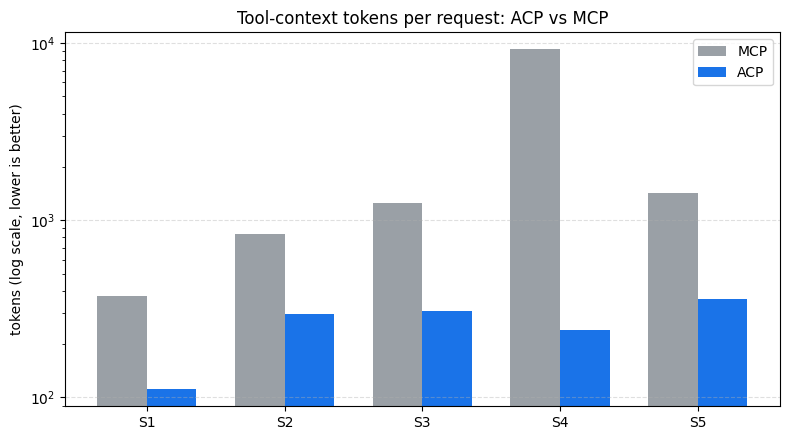
\includegraphics[width=0.9\linewidth]{figures/tokens.png}
\caption{Tool-context tokens per request, log scale. Lower is better.}
\end{figure}

\begin{figure}[h]
\centering
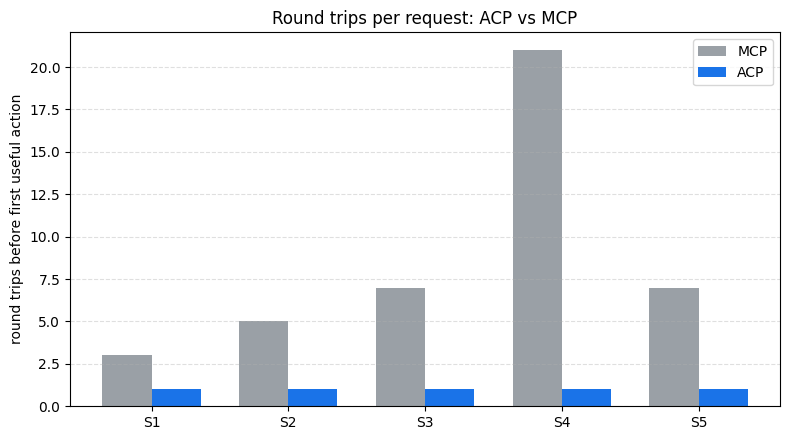
\includegraphics[width=0.9\linewidth]{figures/round_trips.png}
\caption{Round trips before the first useful action.}
\end{figure}

\begin{figure}[h]
\centering
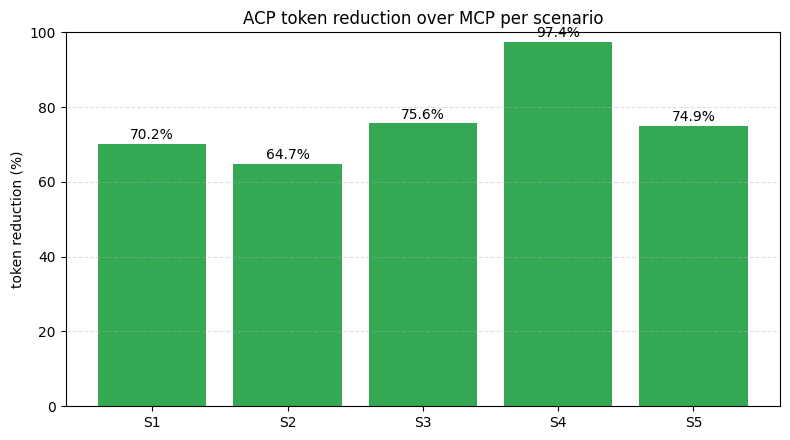
\includegraphics[width=0.9\linewidth]{figures/reduction.png}
\caption{ACP token reduction over MCP per scenario.}
\end{figure}

\subsection{Reproducibility}

The benchmark harness and the MCP-equivalent payload reproducer are open
under Apache 2.0. The committed
\texttt{results/2026-05-02-week3-baseline.json} contains all 250 raw runs.

\subsection{Threats to validity}

All current measurements use \texttt{cl100k\_base}. Models with different
tokenizers and provider-side accounting will report different absolute counts.
The reported percentage reduction is a payload-level result under a fixed
tokenizer; model-specific cost claims require the frontier benchmark described
below. We also discuss MCP descriptor verbosity, compact-schema fidelity, and
network topology in the README of the reference implementation.

\section{Implementation}

The reference implementation is approximately 4{,}500 lines of Go (server,
proxy, registry, builder, MCP source adapter) and 1{,}000 lines of Python
(adapter packages, benchmark harness). Test coverage is 95\% on the Go
core and 96.8\% on the Python tooling, including fuzz coverage for the
schema compactor and dependency resolver, and a live integration test
that exercises the MCP-source-to-ACP-manifest path end to end.

\section{Frontier Benchmark Plan}

The present paper reports a deterministic protocol benchmark. Before claiming
model-specific production gains, we will add a frontier tool-context benchmark
under \texttt{benchmark/frontier/} with BFCL as the primary open standard and
tau-bench / tau$^3$-bench as the secondary multi-turn track.

The planned model matrix has four tiers: a 1M+ context-window model to test
whether long context removes or merely hides descriptor overhead; a medium
frontier tier such as Claude Sonnet and available GPT-5.x medium variants; a
heavy frontier tier such as Claude Opus and the strongest available GPT-5.x /
Gemini Pro-class models; and at least one open or research-licensed
tool-calling model. Exact model IDs will be pinned in result files. If a
colloquial alias is not exposed by a provider API, it will not be used as a
paper claim.

For each selected BFCL task, the harness will construct an MCP
\texttt{tools/list} payload and an ACP registry from the same functions, then
measure descriptor tokens, context utilization, first-action round trips,
provider-reported usage, latency, and BFCL correctness. This separates three
questions that are often conflated: whether ACP reduces protocol overhead,
whether reduced overhead preserves tool-call correctness, and whether frontier
model costs change enough to matter operationally.

\section{Conclusion}

We have introduced ACP, an intent-resolved execution-manifest layer that
sits on top of MCP and other tool sources. Across five representative
workflows ACP cuts tool-context tokens by a measured mean of 76.6\% (range
64.7\%-97.4\%) and reduces round trips before the first useful action
from 3-21 to 1, while leaving the MCP ecosystem unchanged. The reference
implementation is open source.

The next development priorities are a BFCL-based frontier benchmark with pinned
long-context, medium, heavy, and open-model tiers; an embedding-based intent
resolver for production deployments; additional source adapters (REST/OpenAPI,
gRPC reflection, Kubernetes); and a feedback-driven optimizer.

\bibliographystyle{plain}
\bibliography{references}

\end{document}
